\chapter{NỘI DUNG THỰC HIỆN ĐỀ TÀI}

\textit{Chương này trình bày quá trình nghiên cứu, thiết kế và xây dựng hệ thống Secure Chat System with Cryptographic Security. Nội dung bao gồm các công việc đã thực hiện, quy trình phát triển hệ thống, các cơ chế bảo mật được triển khai và kết quả đạt được trong từng giai đoạn thực hiện đề tài.}

\section{Mô tả nội dung thực hiện}

Trong quá trình thực hiện đề tài, nhóm tiến hành nghiên cứu các kiến thức về mật mã học, an toàn thông tin và lập trình ứng dụng Web nhằm xây dựng một hệ thống nhắn tin có khả năng bảo mật dữ liệu trong quá trình truyền thông.

Đề tài được triển khai theo nhiều giai đoạn, từ khảo sát yêu cầu, thiết kế kiến trúc hệ thống, xây dựng giao diện người dùng, lập trình các chức năng chính, tích hợp các thuật toán mật mã cho đến kiểm thử và đánh giá toàn bộ hệ thống.

Các công nghệ và công cụ được sử dụng gồm:

\begin{itemize}
\item Python 3
\item Flask
\item Flask-SocketIO
\item HTML, CSS và JavaScript
\item Cryptography Library
\item Git và GitHub
\item Visual Studio Code
\end{itemize}

Kết quả cuối cùng là một hệ thống nhắn tin thời gian thực tích hợp nhiều cơ chế bảo mật hiện đại như RSA-OAEP, AES-GCM, RSA-PSS, Replay Detector và Session Key Rotation.

\section{Các cuộc tấn công được mô phỏng}

Để đánh giá hiệu quả của các cơ chế bảo mật đã triển khai, nhóm xây dựng nhiều tình huống tấn công thường gặp trong lĩnh vực An toàn thông tin. Mỗi cuộc tấn công đều được thực hiện trực tiếp trên hệ thống nhằm kiểm tra khả năng phát hiện và xử lý của các cơ chế bảo mật.

\subsection{Modify Ciphertext}

Kẻ tấn công thay đổi nội dung bản mã (Ciphertext) trước khi dữ liệu được gửi đến người nhận. Nhờ cơ chế Authentication Tag của AES-GCM, hệ thống có thể phát hiện dữ liệu đã bị thay đổi và từ chối giải mã.

\begin{figure}[H]
\centering
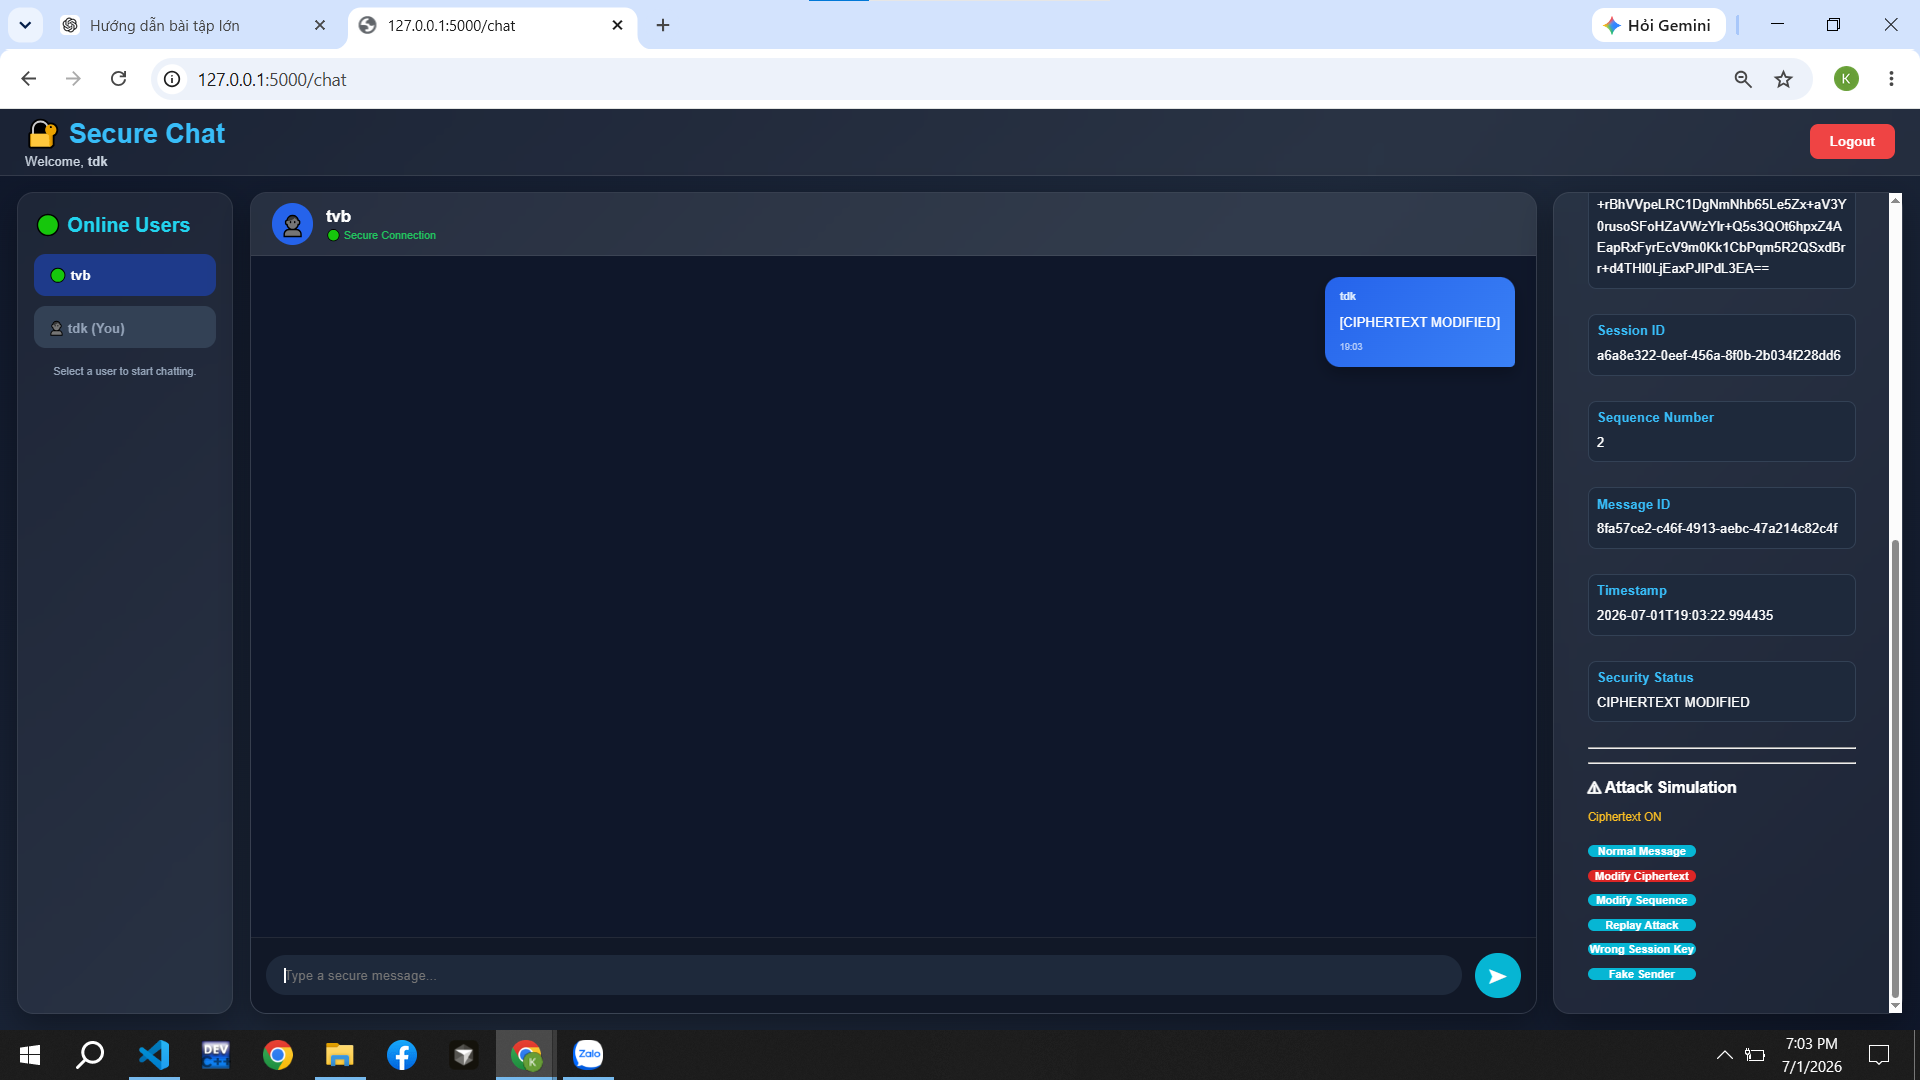
\includegraphics[width=0.95\textwidth]{images/ciphertext_attack.png}
\caption{Mô phỏng tấn công Modify Ciphertext}
\label{fig:ciphertext_attack}
\Nguon{Trần Khiêm}
\end{figure}

\subsection{Replay Attack}

Replay Attack là hình thức gửi lại một gói tin đã được truyền trước đó nhằm đánh lừa hệ thống. Replay Detector sử dụng Message ID để phát hiện các gói tin đã từng được xử lý và tự động từ chối các gói tin bị phát lại.

\begin{figure}[H]
\centering
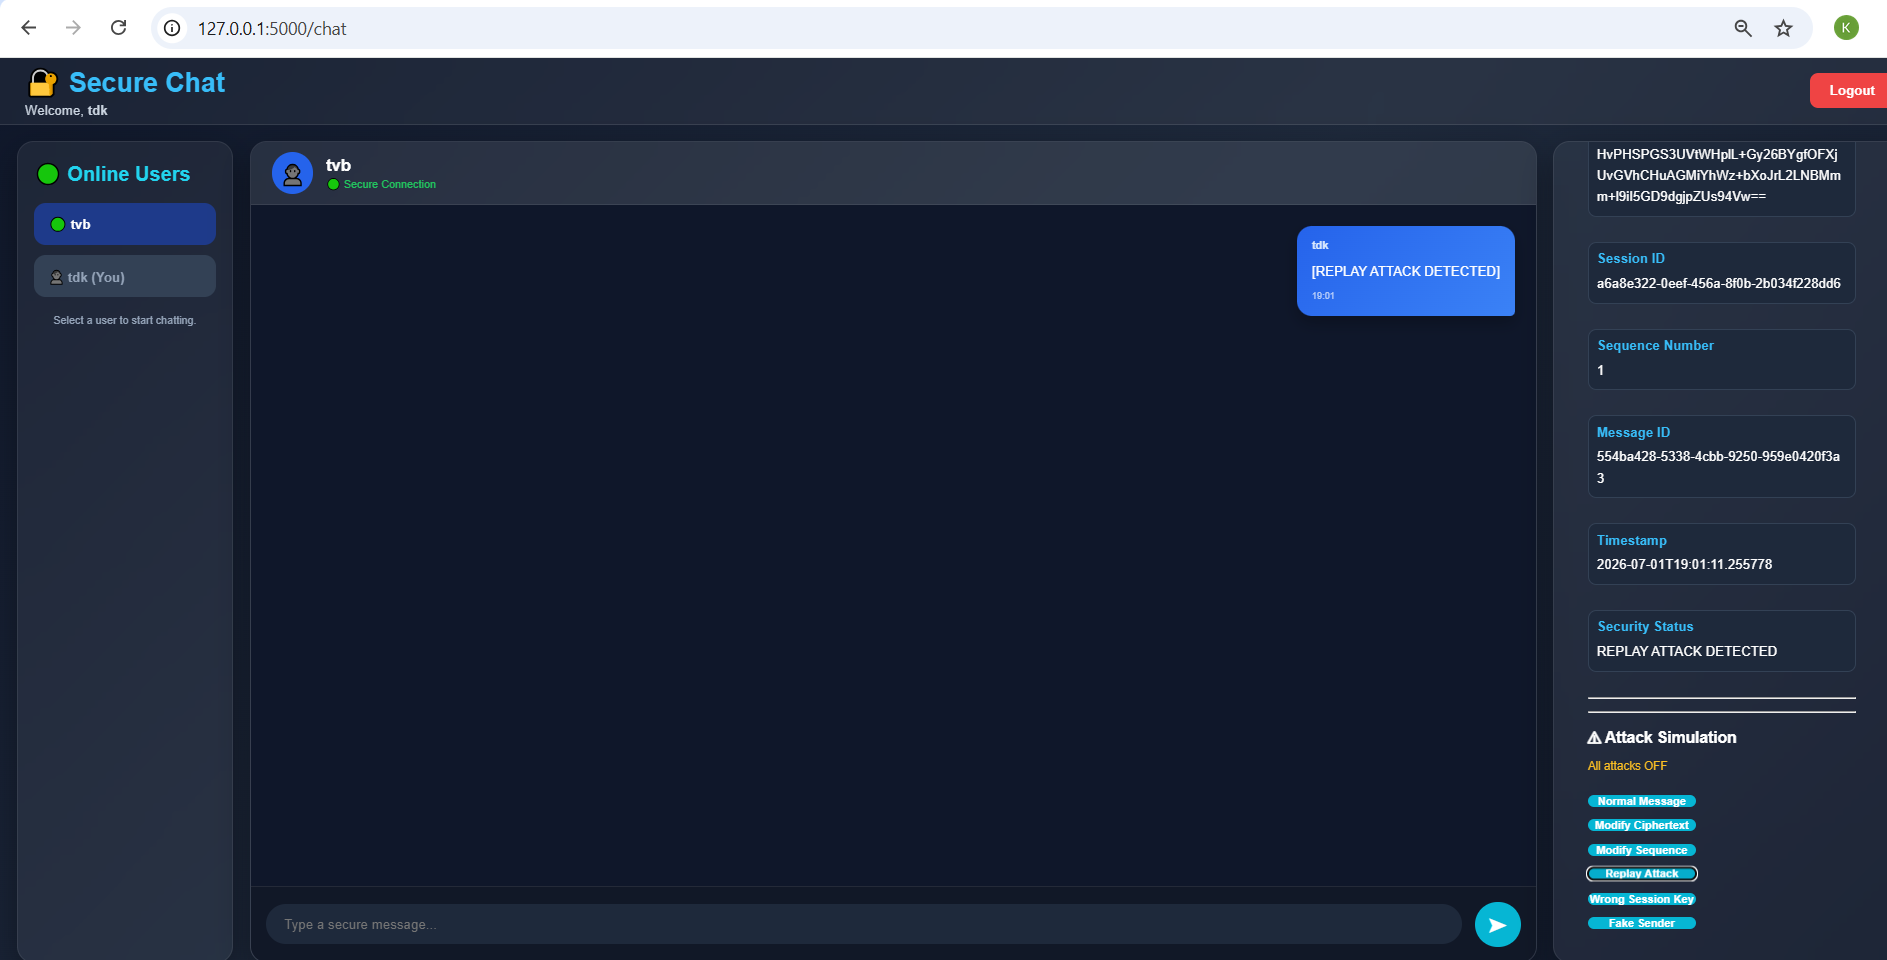
\includegraphics[width=0.95\textwidth]{images/replay_attack.png}
\caption{Mô phỏng Replay Attack}
\label{fig:replay_attack}
\Nguon{Trần Khiêm}
\end{figure}

\subsection{Wrong Session Key}

Trong tình huống này, người nhận sử dụng một Session Key không đúng để giải mã dữ liệu. Do khóa phiên không khớp với khóa dùng để mã hóa nên quá trình giải mã thất bại và hệ thống sinh cảnh báo.

\begin{figure}[H]
\centering
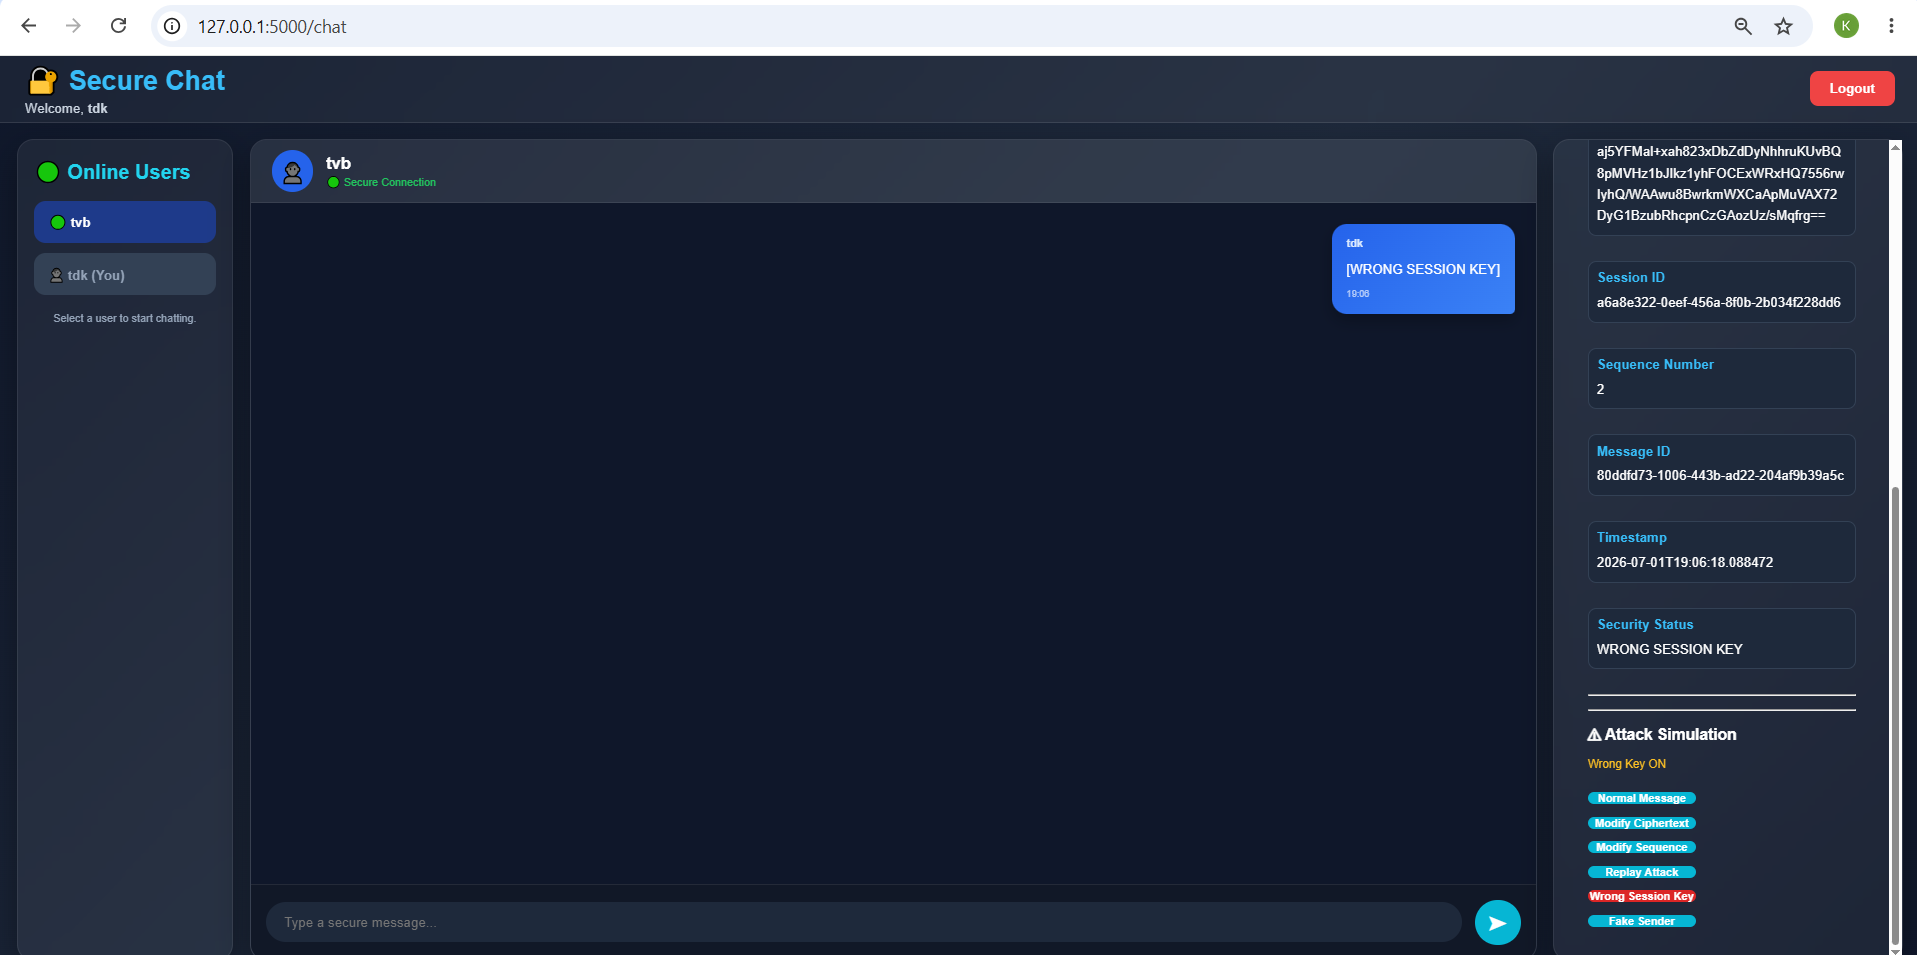
\includegraphics[width=0.95\textwidth]{images/wrong_key_attack.png}
\caption{Mô phỏng sử dụng Session Key không hợp lệ}
\label{fig:wrong_key_attack}
\Nguon{Trần Khiêm}
\end{figure}

\subsection{Fake Sender}

Kẻ tấn công thay đổi thông tin người gửi hoặc cố gắng giả mạo chữ ký số. Nhờ cơ chế xác thực RSA-PSS, hệ thống kiểm tra chữ ký trước khi giải mã và phát hiện ngay hành vi giả mạo.

\begin{figure}[H]
\centering
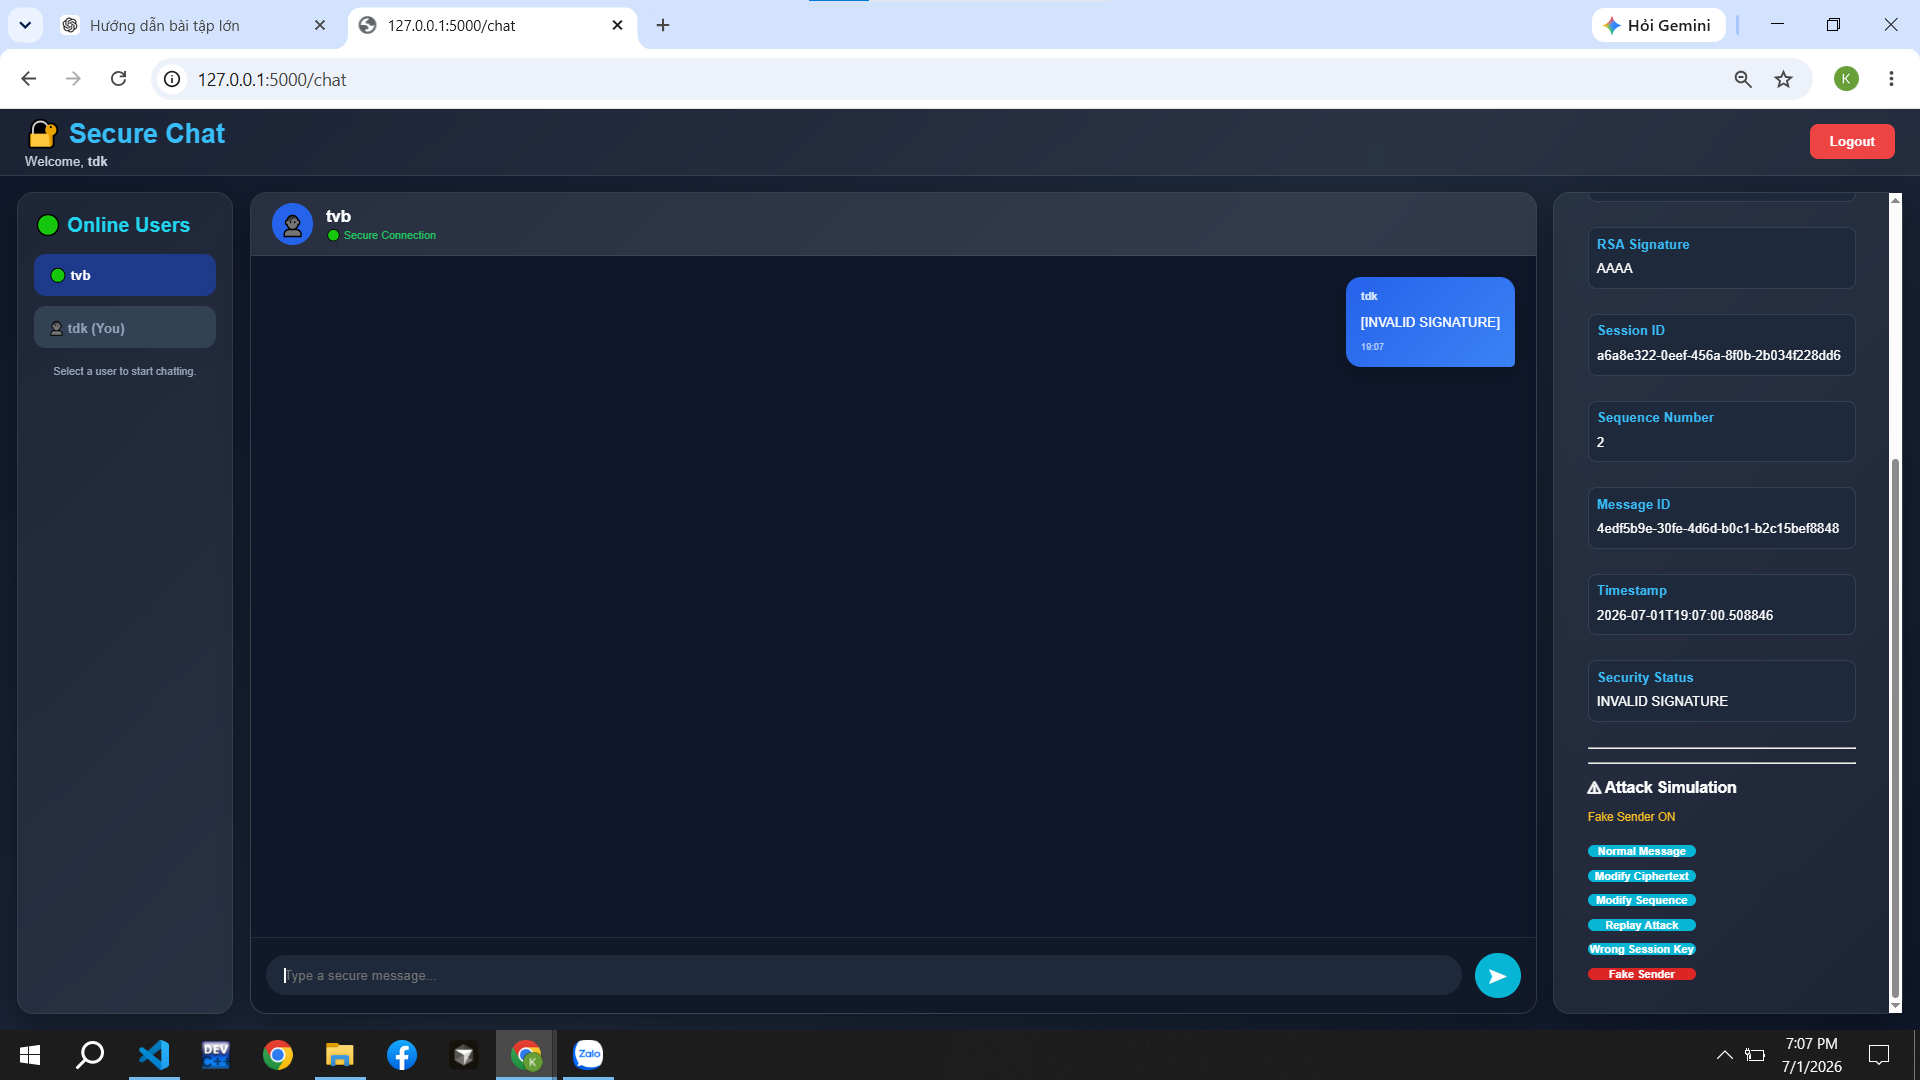
\includegraphics[width=0.95\textwidth]{images/fake_sender_attack.png}
\caption{Mô phỏng tấn công Fake Sender}
\label{fig:fake_sender_attack}
\Nguon{Trần Khiêm}
\end{figure}

\subsection{Modify Sequence Number}

Sequence Number được sử dụng để kiểm tra thứ tự của các gói tin trong một phiên làm việc. Khi số thứ tự bị thay đổi, hệ thống phát hiện sự bất thường và cảnh báo nguy cơ tấn công hoặc dữ liệu bị chỉnh sửa.

\begin{figure}[H]
\centering
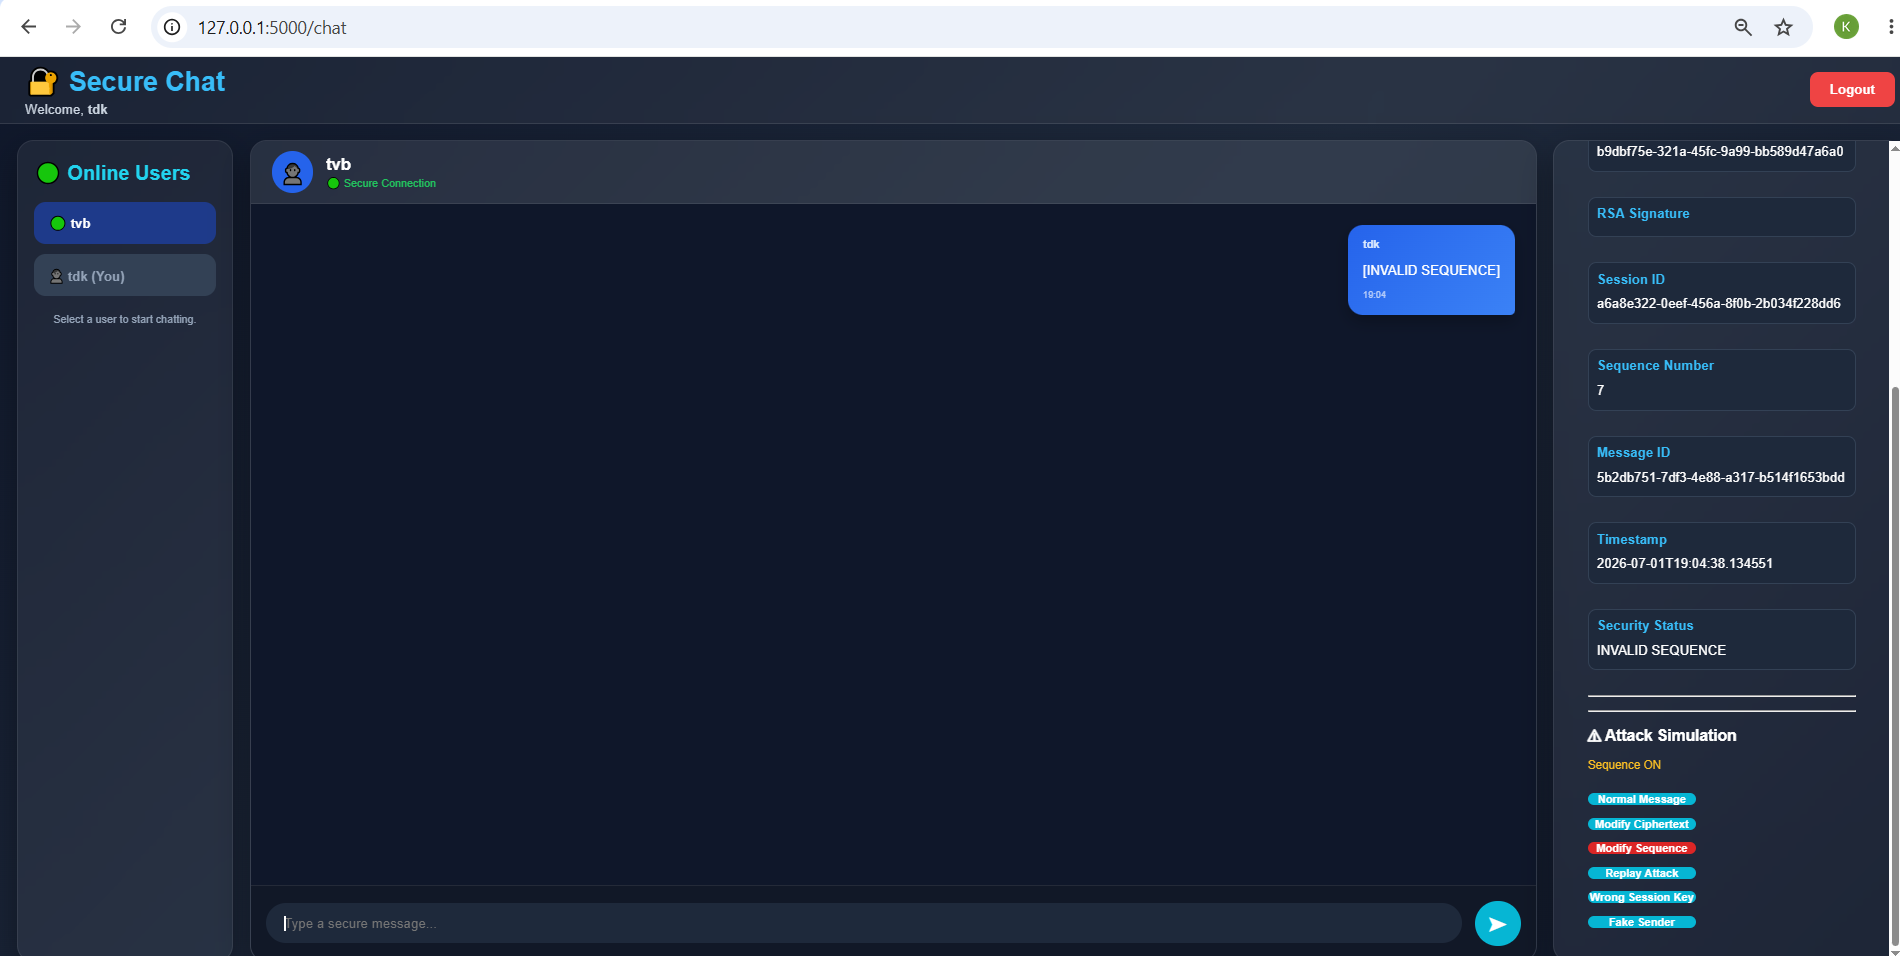
\includegraphics[width=0.95\textwidth]{images/sequence_attack.png}
\caption{Mô phỏng tấn công Modify Sequence Number}
\label{fig:sequence_attack}
\Nguon{Trần Khiêm}
\end{figure}

Sau khi thực hiện các tình huống trên, hệ thống đều đưa ra cảnh báo tương ứng trên bảng Security Information. Điều này chứng minh các cơ chế bảo mật được triển khai có khả năng phát hiện hiệu quả các hành vi tấn công và đảm bảo tính bí mật, toàn vẹn cũng như xác thực của dữ liệu trong quá trình truyền thông.

\section{Các công việc đã thực hiện}

Trong quá trình xây dựng hệ thống, nhóm đã hoàn thành các nội dung chính sau:

\begin{itemize}
\item Phân tích yêu cầu và thiết kế kiến trúc hệ thống.
\item Thiết kế giao diện đăng ký, đăng nhập và màn hình nhắn tin.
\item Xây dựng chức năng đăng ký và đăng nhập người dùng.
\item Xây dựng chức năng nhắn tin thời gian thực bằng Flask-SocketIO.
\item Tích hợp RSA-OAEP để trao đổi khóa phiên.
\item Tích hợp AES-GCM để mã hóa và giải mã nội dung tin nhắn.
\item Tích hợp RSA-PSS để ký số và xác thực người gửi.
\item Xây dựng Replay Detector.
\item Quản lý Session ID, Message ID và Sequence Number.
\item Cài đặt Session Key Rotation.
\item Thiết kế bảng Security Information.
\item Xây dựng các chức năng mô phỏng tấn công.
\item Kiểm thử và đánh giá toàn bộ hệ thống.
\end{itemize}

\section{Quy trình phát triển hệ thống}

Quá trình phát triển hệ thống được thực hiện theo các bước sau:

\begin{enumerate}
\item Khảo sát yêu cầu và xác định mục tiêu của hệ thống.
\item Thiết kế giao diện và kiến trúc tổng thể.
\item Xây dựng các chức năng cơ bản.
\item Tích hợp các thuật toán mật mã.
\item Hoàn thiện cơ chế bảo mật.
\item Kiểm thử và tối ưu hệ thống.
\end{enumerate}

\section{Chi tiết quá trình thực hiện}

\begin{longtable}{|c|p{3cm}|p{6cm}|p{4cm}|}
\caption{Quá trình thực hiện đề tài}
\label{tab:qua-trinh-thuc-hien}\\

\hline
\textbf{Giai đoạn} &
\textbf{Thời gian} &
\textbf{Nội dung thực hiện} &
\textbf{Kết quả đạt được}\\
\hline
\endfirsthead

\hline
\textbf{Giai đoạn} &
\textbf{Thời gian} &
\textbf{Nội dung thực hiện} &
\textbf{Kết quả đạt được}\\
\hline
\endhead

1 &
Tuần 1 &
Khảo sát yêu cầu đề tài, nghiên cứu Flask, Socket.IO và các thuật toán mật mã RSA, AES.
&
Xây dựng định hướng phát triển hệ thống.
\\
\hline

2 &
Tuần 2 &
Thiết kế giao diện và kiến trúc hệ thống; xây dựng chức năng đăng ký và đăng nhập.
&
Hoàn thành giao diện Login và Register.
\\
\hline

3 &
Tuần 3 &
Xây dựng chức năng nhắn tin thời gian thực; tích hợp RSA-OAEP, AES-GCM và RSA-PSS.
&
Hoàn thiện chức năng gửi và nhận tin nhắn bảo mật.
\\
\hline

4 &
Tuần 4 &
Xây dựng Replay Detector, Session Manager, Session Key Rotation và bảng Security Information.
&
Hoàn thiện các cơ chế bảo mật của hệ thống.
\\
\hline

5 &
Tuần 5 &
Xây dựng các chức năng mô phỏng tấn công gồm Modify Ciphertext, Replay Attack, Wrong Session Key, Fake Sender và Modify Sequence Number.
&
Hoàn thành các chức năng kiểm thử an toàn thông tin.
\\
\hline

6 &
Tuần 6 &
Kiểm thử toàn bộ hệ thống, sửa lỗi và tối ưu chương trình.
&
Hoàn thiện phiên bản cuối cùng của hệ thống.
\\
\hline

\end{longtable}

\begin{flushright}
\textit{Nguồn: Nhóm tác giả tổng hợp}
\end{flushright}